\documentclass[]{article}
\usepackage{lmodern}
\usepackage{amssymb,amsmath}
\usepackage{ifxetex,ifluatex}
\usepackage{fixltx2e} % provides \textsubscript
\ifnum 0\ifxetex 1\fi\ifluatex 1\fi=0 % if pdftex
  \usepackage[T1]{fontenc}
  \usepackage[utf8]{inputenc}
\else % if luatex or xelatex
  \ifxetex
    \usepackage{mathspec}
  \else
    \usepackage{fontspec}
  \fi
  \defaultfontfeatures{Ligatures=TeX,Scale=MatchLowercase}
\fi
% use upquote if available, for straight quotes in verbatim environments
\IfFileExists{upquote.sty}{\usepackage{upquote}}{}
% use microtype if available
\IfFileExists{microtype.sty}{%
\usepackage{microtype}
\UseMicrotypeSet[protrusion]{basicmath} % disable protrusion for tt fonts
}{}
\usepackage[margin=1in]{geometry}
\usepackage{hyperref}
\hypersetup{unicode=true,
            pdftitle={INApreliminary - Analysis of the role of individual nodes in sampling epidemic spread v6},
            pdfborder={0 0 0},
            breaklinks=true}
\urlstyle{same}  % don't use monospace font for urls
\usepackage{color}
\usepackage{fancyvrb}
\newcommand{\VerbBar}{|}
\newcommand{\VERB}{\Verb[commandchars=\\\{\}]}
\DefineVerbatimEnvironment{Highlighting}{Verbatim}{commandchars=\\\{\}}
% Add ',fontsize=\small' for more characters per line
\usepackage{framed}
\definecolor{shadecolor}{RGB}{248,248,248}
\newenvironment{Shaded}{\begin{snugshade}}{\end{snugshade}}
\newcommand{\KeywordTok}[1]{\textcolor[rgb]{0.13,0.29,0.53}{\textbf{#1}}}
\newcommand{\DataTypeTok}[1]{\textcolor[rgb]{0.13,0.29,0.53}{#1}}
\newcommand{\DecValTok}[1]{\textcolor[rgb]{0.00,0.00,0.81}{#1}}
\newcommand{\BaseNTok}[1]{\textcolor[rgb]{0.00,0.00,0.81}{#1}}
\newcommand{\FloatTok}[1]{\textcolor[rgb]{0.00,0.00,0.81}{#1}}
\newcommand{\ConstantTok}[1]{\textcolor[rgb]{0.00,0.00,0.00}{#1}}
\newcommand{\CharTok}[1]{\textcolor[rgb]{0.31,0.60,0.02}{#1}}
\newcommand{\SpecialCharTok}[1]{\textcolor[rgb]{0.00,0.00,0.00}{#1}}
\newcommand{\StringTok}[1]{\textcolor[rgb]{0.31,0.60,0.02}{#1}}
\newcommand{\VerbatimStringTok}[1]{\textcolor[rgb]{0.31,0.60,0.02}{#1}}
\newcommand{\SpecialStringTok}[1]{\textcolor[rgb]{0.31,0.60,0.02}{#1}}
\newcommand{\ImportTok}[1]{#1}
\newcommand{\CommentTok}[1]{\textcolor[rgb]{0.56,0.35,0.01}{\textit{#1}}}
\newcommand{\DocumentationTok}[1]{\textcolor[rgb]{0.56,0.35,0.01}{\textbf{\textit{#1}}}}
\newcommand{\AnnotationTok}[1]{\textcolor[rgb]{0.56,0.35,0.01}{\textbf{\textit{#1}}}}
\newcommand{\CommentVarTok}[1]{\textcolor[rgb]{0.56,0.35,0.01}{\textbf{\textit{#1}}}}
\newcommand{\OtherTok}[1]{\textcolor[rgb]{0.56,0.35,0.01}{#1}}
\newcommand{\FunctionTok}[1]{\textcolor[rgb]{0.00,0.00,0.00}{#1}}
\newcommand{\VariableTok}[1]{\textcolor[rgb]{0.00,0.00,0.00}{#1}}
\newcommand{\ControlFlowTok}[1]{\textcolor[rgb]{0.13,0.29,0.53}{\textbf{#1}}}
\newcommand{\OperatorTok}[1]{\textcolor[rgb]{0.81,0.36,0.00}{\textbf{#1}}}
\newcommand{\BuiltInTok}[1]{#1}
\newcommand{\ExtensionTok}[1]{#1}
\newcommand{\PreprocessorTok}[1]{\textcolor[rgb]{0.56,0.35,0.01}{\textit{#1}}}
\newcommand{\AttributeTok}[1]{\textcolor[rgb]{0.77,0.63,0.00}{#1}}
\newcommand{\RegionMarkerTok}[1]{#1}
\newcommand{\InformationTok}[1]{\textcolor[rgb]{0.56,0.35,0.01}{\textbf{\textit{#1}}}}
\newcommand{\WarningTok}[1]{\textcolor[rgb]{0.56,0.35,0.01}{\textbf{\textit{#1}}}}
\newcommand{\AlertTok}[1]{\textcolor[rgb]{0.94,0.16,0.16}{#1}}
\newcommand{\ErrorTok}[1]{\textcolor[rgb]{0.64,0.00,0.00}{\textbf{#1}}}
\newcommand{\NormalTok}[1]{#1}
\usepackage{graphicx,grffile}
\makeatletter
\def\maxwidth{\ifdim\Gin@nat@width>\linewidth\linewidth\else\Gin@nat@width\fi}
\def\maxheight{\ifdim\Gin@nat@height>\textheight\textheight\else\Gin@nat@height\fi}
\makeatother
% Scale images if necessary, so that they will not overflow the page
% margins by default, and it is still possible to overwrite the defaults
% using explicit options in \includegraphics[width, height, ...]{}
\setkeys{Gin}{width=\maxwidth,height=\maxheight,keepaspectratio}
\IfFileExists{parskip.sty}{%
\usepackage{parskip}
}{% else
\setlength{\parindent}{0pt}
\setlength{\parskip}{6pt plus 2pt minus 1pt}
}
\setlength{\emergencystretch}{3em}  % prevent overfull lines
\providecommand{\tightlist}{%
  \setlength{\itemsep}{0pt}\setlength{\parskip}{0pt}}
\setcounter{secnumdepth}{0}
% Redefines (sub)paragraphs to behave more like sections
\ifx\paragraph\undefined\else
\let\oldparagraph\paragraph
\renewcommand{\paragraph}[1]{\oldparagraph{#1}\mbox{}}
\fi
\ifx\subparagraph\undefined\else
\let\oldsubparagraph\subparagraph
\renewcommand{\subparagraph}[1]{\oldsubparagraph{#1}\mbox{}}
\fi

%%% Use protect on footnotes to avoid problems with footnotes in titles
\let\rmarkdownfootnote\footnote%
\def\footnote{\protect\rmarkdownfootnote}

%%% Change title format to be more compact
\usepackage{titling}

% Create subtitle command for use in maketitle
\newcommand{\subtitle}[1]{
  \posttitle{
    \begin{center}\large#1\end{center}
    }
}

\setlength{\droptitle}{-2em}

  \title{INApreliminary - Analysis of the role of individual nodes in sampling
epidemic spread v6}
    \pretitle{\vspace{\droptitle}\centering\huge}
  \posttitle{\par}
    \author{}
    \preauthor{}\postauthor{}
    \date{}
    \predate{}\postdate{}
  

\begin{document}
\maketitle

K. A. Garrett, University of Florida

\subsection{Impact network analysis}\label{impact-network-analysis}

Impact network analysis (INA) is designed to address multiple aspects of
linked socioeconomic networks (spread of ideas, money, influence, etc.)
and biophysical networks (spread of new varieties, certified seed,
pathogens, pests, etc.).

The functions introduced here are part of an R package under
development, ``INA''. INA is the analysis of how technologies affect
regional outcomes, such as productivity or disease incidence, through
their effects on linked socioeconomic and biophysical networks (Garrett
2018).

Garrett KA, 2018. Impact network analysis: evaluating the success of
interventions. PeerJ Preprints 6, e27037v1
\url{https://doi.org/10.7287/peerj.preprints.v1}.

\subsection{Risk-based surveillance strategies, as part of an impact
network
analysis}\label{risk-based-surveillance-strategies-as-part-of-an-impact-network-analysis}

The example given here addresses identifying the best locations in a
network for sampling to quickly detect a spreading pathogen (or
spreading new variety, for example). A node is better for sampling if
the pathogen is likely to be detected at that node before the pathogen
has spread very far through the network. For example, an isolated node
would be a poor sampling choice because the pathogen could spread widely
before it reaches the isolated node.

The functions for this analysis can also take into account information
about where the pathogen is more likely to enter the network. For
example, nodes with little information available through communication
networks may be more likely to be vulnerable to being entry points for
pathogens.

\section{Getting the INApreliminary package from
GitHub}\label{getting-the-inapreliminary-package-from-github}

An updated version of INApreliminary will be available on GitHub soon,
and a complete version with multiple types of scenario analyses will be
available later this year.

The examples below include creation of the functions that will later be
available as part of INApreliminary.

\subsection{A simple example}\label{a-simple-example}

Consider a simple adjacency matrix, which will be used to illustrate the
functions.

\begin{Shaded}
\begin{Highlighting}[]
\KeywordTok{library}\NormalTok{(}\StringTok{'igraph'}\NormalTok{)}
\NormalTok{Amat <-}\StringTok{ }\KeywordTok{matrix}\NormalTok{(}\KeywordTok{c}\NormalTok{(}\DecValTok{1}\NormalTok{,}\DecValTok{0}\NormalTok{,}\DecValTok{0}\NormalTok{,}\DecValTok{0}\NormalTok{,}\DecValTok{1}\NormalTok{,}\DecValTok{1}\NormalTok{,}\DecValTok{0}\NormalTok{,}\DecValTok{0}\NormalTok{,}\DecValTok{0}\NormalTok{,}\DecValTok{1}\NormalTok{,}\DecValTok{1}\NormalTok{,}\DecValTok{0}\NormalTok{,}\DecValTok{1}\NormalTok{,}\DecValTok{1}\NormalTok{,}\DecValTok{1}\NormalTok{,}\DecValTok{1}\NormalTok{),}\DataTypeTok{nrow=}\DecValTok{4}\NormalTok{,}\DataTypeTok{ncol=}\DecValTok{4}\NormalTok{)}
\NormalTok{Amati <-}\StringTok{ }\KeywordTok{graph.adjacency}\NormalTok{(Amat)}
\KeywordTok{plot}\NormalTok{(Amati)}
\end{Highlighting}
\end{Shaded}

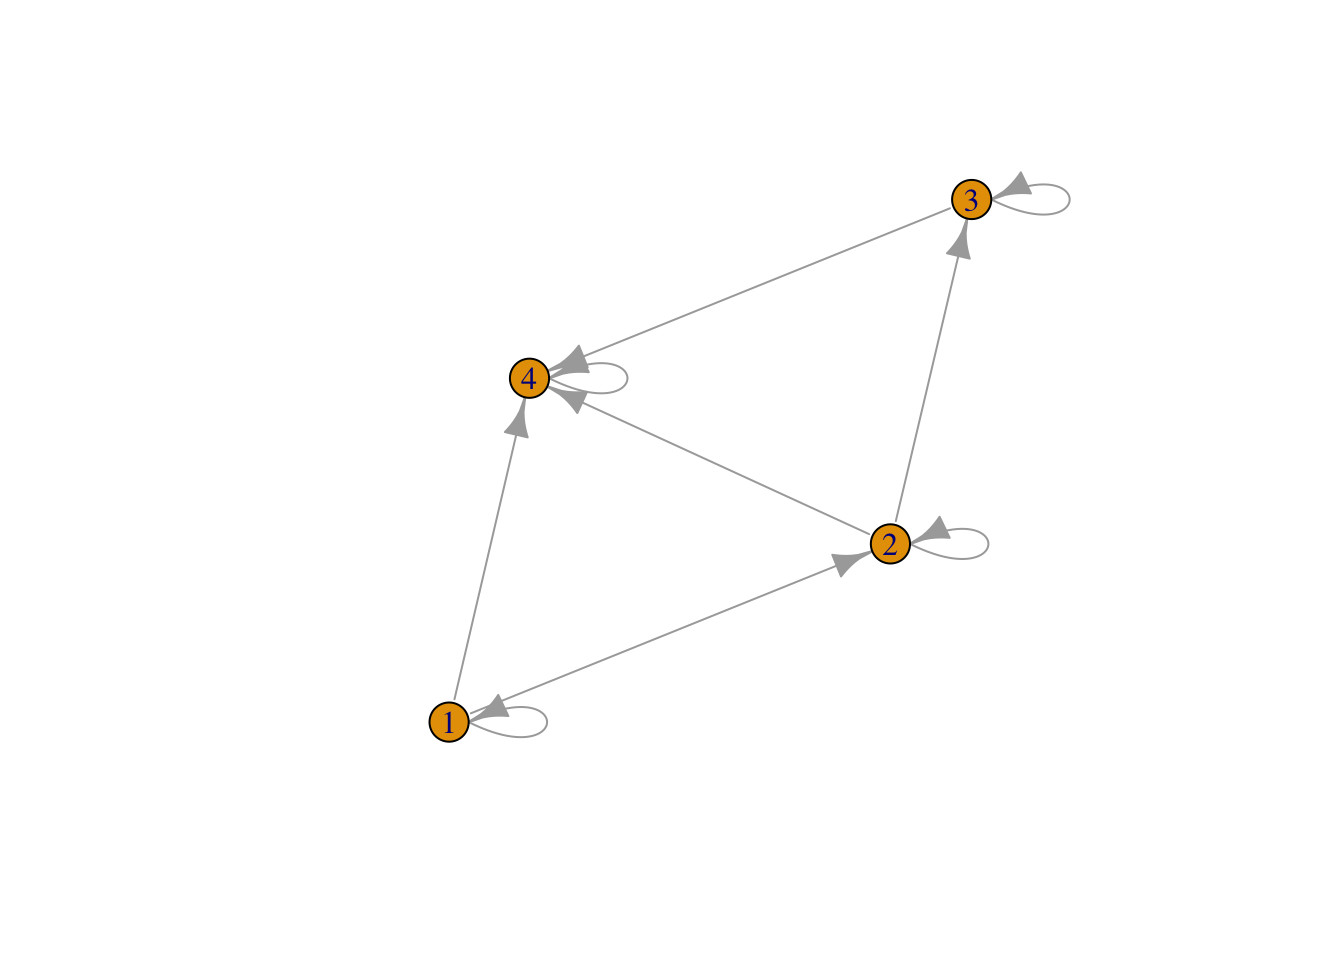
\includegraphics{INA_files/figure-latex/unnamed-chunk-1-1.pdf}

\begin{Shaded}
\begin{Highlighting}[]
\NormalTok{sAmat <-}\StringTok{ }\NormalTok{Amat }\OperatorTok{*}\StringTok{ }\FloatTok{0.7} \CommentTok{# each potential link has probability 0.7 of existing - this will sometimes be useful}
\end{Highlighting}
\end{Shaded}

\subsection{Illustration}\label{illustration}

For a single selected starting node, the invdetf function yields a
vector of the number of nodes invaded for each sampling node by the time
invasion reaches (is detected at) that sampling node, and the time step
of first invasion at the sampling node - for one simulation.

The following code creates the function invdetf.

\begin{Shaded}
\begin{Highlighting}[]
\NormalTok{invdetf <-}\StringTok{ }\ControlFlowTok{function}\NormalTok{(adjmat, start.choice, }\DataTypeTok{stoch=}\NormalTok{F)\{}

\NormalTok{  ### for all three functions, need to add in the definitions for the input variables...}
  
\NormalTok{  dimL <-}\StringTok{ }\KeywordTok{dim}\NormalTok{(adjmat)[}\DecValTok{1}\NormalTok{] }\CommentTok{# number of rows of adjacency matrix}
\NormalTok{  t1 <-}\StringTok{ }\KeywordTok{matrix}\NormalTok{( }\DecValTok{0} \OperatorTok{*}\StringTok{ }\DecValTok{1}\OperatorTok{:}\NormalTok{dimL, }\DataTypeTok{nrow=}\DecValTok{1}\NormalTok{)}
\NormalTok{  t1[,start.choice] <-}\StringTok{ }\DecValTok{1} \CommentTok{# starting node labelled 1}
  
  \CommentTok{# if a stochastic model, generate the adjacency matrix for this simulation}
    \CommentTok{# if stochastic, assumes the adjacency matrix is made up of probabilities}

  \ControlFlowTok{if}\NormalTok{(stoch)\{ }\CommentTok{# need to think about the temporal resolution of stochasticity...}
\NormalTok{    adjmat <-}\StringTok{ }\NormalTok{(}\KeywordTok{matrix}\NormalTok{(}\KeywordTok{runif}\NormalTok{(dimL}\OperatorTok{^}\DecValTok{2}\NormalTok{), }\DataTypeTok{ncol=}\NormalTok{dimL) }\OperatorTok{<}\StringTok{ }\NormalTok{adjmat)}
\NormalTok{  \}}

  \CommentTok{# generate the infection status for each node at each time point until spread stops}

\NormalTok{  outmat <-}\StringTok{ }\NormalTok{t1}
\NormalTok{  infcount.pre <-}\StringTok{ }\DecValTok{1}
\NormalTok{  infcount.post <-}\StringTok{ }\OperatorTok{-}\DecValTok{9} \CommentTok{# perhaps improve structure}

  \ControlFlowTok{while}\NormalTok{(}\KeywordTok{sum}\NormalTok{(t1) }\OperatorTok{<}\StringTok{ }\NormalTok{dimL }\OperatorTok{&}\StringTok{ }\NormalTok{infcount.pre }\OperatorTok{!=}\StringTok{ }\NormalTok{infcount.post)\{}
\NormalTok{    infcount.pre <-}\StringTok{ }\KeywordTok{sum}\NormalTok{(t1) }\CommentTok{# perhaps change to infcount.pre <- infcount.post}
\NormalTok{    t1 <-}\StringTok{ }\KeywordTok{as.numeric}\NormalTok{(t1 }\OperatorTok\StringTok{ }\NormalTok{adjmat }\OperatorTok{>}\StringTok{ }\DecValTok{0}\NormalTok{)}
\NormalTok{    infcount.post <-}\StringTok{ }\KeywordTok{sum}\NormalTok{(t1)}
\NormalTok{    outmat <-}\StringTok{ }\KeywordTok{rbind}\NormalTok{(outmat,t1) }\CommentTok{# row i is the ith time point}
\NormalTok{  \}}

  \CommentTok{# find the num infected for each single sampling node, }
     \CommentTok{# assuming infected node stays infected...}
    \CommentTok{# consider whether to set diag...}

  \CommentTok{# find the number of nodes infected at each time}
\NormalTok{  inft <-}\StringTok{ }\KeywordTok{rowSums}\NormalTok{(outmat)}

  \CommentTok{# find the first time each node is invaded, and number of nodes infected at that time}
\NormalTok{  firstt <-}\StringTok{ }\OperatorTok{-}\DecValTok{99} \OperatorTok{+}\StringTok{ }\DecValTok{0}\OperatorTok{*}\DecValTok{1}\OperatorTok{:}\NormalTok{dimL }\CommentTok{# first time each node is invaded}
\NormalTok{  numt <-}\StringTok{ }\NormalTok{firstt }\CommentTok{# number of nodes infected at that time}

  \ControlFlowTok{for}\NormalTok{ (i }\ControlFlowTok{in} \DecValTok{1}\OperatorTok{:}\NormalTok{dimL)\{ }\CommentTok{# col i is the ith sample node}

    \ControlFlowTok{if}\NormalTok{ (}\KeywordTok{sum}\NormalTok{(outmat[,i] }\OperatorTok{>}\StringTok{ }\DecValTok{0}\NormalTok{))\{ }\CommentTok{# if node i ever gets infected}
\NormalTok{      firstt[i] <-}\StringTok{ }\KeywordTok{min}\NormalTok{(}\KeywordTok{which}\NormalTok{(outmat[,i] }\OperatorTok{>}\StringTok{ }\DecValTok{0}\NormalTok{)) }\CommentTok{# first time}
\NormalTok{      numt[i] <-}\StringTok{ }\NormalTok{inft[firstt[i]] }\CommentTok{# how many nodes at that time}
\NormalTok{    \}}
    \ControlFlowTok{else}\NormalTok{ \{}
\NormalTok{      firstt[i] <-}\StringTok{ }\OtherTok{Inf}
\NormalTok{      numt[i] <-}\StringTok{ }\KeywordTok{max}\NormalTok{(inft)}
\NormalTok{    \}}

\NormalTok{  \}}

  \CommentTok{# for each node, time first invaded and number of nodes infected at that time}
\NormalTok{  sampnode <-}\StringTok{ }\KeywordTok{cbind}\NormalTok{(firstt, numt)}

  \KeywordTok{list}\NormalTok{(}\DataTypeTok{outmat=}\NormalTok{outmat, }\DataTypeTok{sampnode=}\NormalTok{sampnode)}
\NormalTok{\}}
\end{Highlighting}
\end{Shaded}

The output is two matrices. The first matrix gives the infection status
for each node (column) at each time point (row) until there is no
further spread. The second matrix gives, for each node (row), the time
until infection (column 1) and the number of nodes infected when at that
time (column 2).

\begin{Shaded}
\begin{Highlighting}[]
\KeywordTok{invdetf}\NormalTok{(}\DataTypeTok{adjmat=}\NormalTok{Amat, }\DataTypeTok{start.choice=}\DecValTok{2}\NormalTok{) }\CommentTok{# in this case, the second node was selected as the starting point}
\end{Highlighting}
\end{Shaded}

\begin{verbatim}
## $outmat
##    [,1] [,2] [,3] [,4]
##       0    1    0    0
## t1    0    1    1    1
## t1    0    1    1    1
## 
## $sampnode
##      firstt numt
## [1,]    Inf    3
## [2,]      1    1
## [3,]      2    3
## [4,]      2    3
\end{verbatim}

\begin{Shaded}
\begin{Highlighting}[]
\KeywordTok{invdetf}\NormalTok{(}\DataTypeTok{adjmat=}\NormalTok{sAmat, }\DataTypeTok{start.choice=}\DecValTok{2}\NormalTok{,}\DataTypeTok{stoch=}\NormalTok{T) }\CommentTok{# stochastic version}
\end{Highlighting}
\end{Shaded}

\begin{verbatim}
## $outmat
##    [,1] [,2] [,3] [,4]
##       0    1    0    0
## t1    0    0    1    0
## 
## $sampnode
##      firstt numt
## [1,]    Inf    1
## [2,]      1    1
## [3,]      2    1
## [4,]    Inf    1
\end{verbatim}

The function allstartf summarizes this analysis across all potential
starting points. The following code creates allstartf.

\begin{Shaded}
\begin{Highlighting}[]
\NormalTok{allstartf <-}\StringTok{ }\ControlFlowTok{function}\NormalTok{(adjmat2, }\DataTypeTok{stoch2=}\NormalTok{F)\{}

\NormalTok{  dimL <-}\StringTok{ }\KeywordTok{dim}\NormalTok{(adjmat2)[}\DecValTok{1}\NormalTok{]}

\NormalTok{  alloutmat <-}\StringTok{ }\KeywordTok{matrix}\NormalTok{(}\OperatorTok{-}\DecValTok{99}\NormalTok{, }\DataTypeTok{ncol=}\NormalTok{dimL, }\DataTypeTok{nrow=}\NormalTok{dimL)}

  \ControlFlowTok{for}\NormalTok{ (i }\ControlFlowTok{in} \DecValTok{1}\OperatorTok{:}\NormalTok{dimL) \{}
\NormalTok{    alloutmat[i,] <-}\StringTok{ }\KeywordTok{invdetf}\NormalTok{(}\DataTypeTok{adjmat=}\NormalTok{adjmat2, }\DataTypeTok{start.choice=}\NormalTok{i, }\DataTypeTok{stoch=}\NormalTok{stoch2)}\OperatorTok{$}\NormalTok{sampnode[,}\DecValTok{2}\NormalTok{]}
\NormalTok{  \}}

\NormalTok{alloutmat}
\NormalTok{\}}
\end{Highlighting}
\end{Shaded}

The output is a matrix with entries being the number of nodes infected
by the time an invasion is detected at each potential sampling node.
Rows in this matrix are potential introduction nodes and columns are
potential sampling nodes. For the stochastic case, the result is based
on only one simulation (at this point in the analysis).

Note that the diagonal contains ones, because when a node is both the
starting point and the sampling point, the epidemic will only have
reached one node before detection.

\begin{Shaded}
\begin{Highlighting}[]
\KeywordTok{allstartf}\NormalTok{(}\DataTypeTok{adjmat2=}\NormalTok{Amat)}
\end{Highlighting}
\end{Shaded}

\begin{verbatim}
##      [,1] [,2] [,3] [,4]
## [1,]    1    3    4    3
## [2,]    3    1    3    3
## [3,]    2    2    1    2
## [4,]    1    1    1    1
\end{verbatim}

\begin{Shaded}
\begin{Highlighting}[]
\KeywordTok{allstartf}\NormalTok{(}\DataTypeTok{adjmat2=}\NormalTok{sAmat, }\DataTypeTok{stoch2=}\NormalTok{T)}
\end{Highlighting}
\end{Shaded}

\begin{verbatim}
##      [,1] [,2] [,3] [,4]
## [1,]    1    2    2    2
## [2,]    3    1    3    3
## [3,]    2    2    1    2
## [4,]    1    1    1    1
\end{verbatim}

The function multisimf performs the same analysis, for the specified
number of simulations.

\begin{Shaded}
\begin{Highlighting}[]
\NormalTok{multisimf <-}\StringTok{ }\ControlFlowTok{function}\NormalTok{(adjmat3, }\DataTypeTok{stoch3=}\NormalTok{F, }\DataTypeTok{nsim=}\DecValTok{1}\NormalTok{) \{}

\NormalTok{  dimL <-}\StringTok{ }\KeywordTok{dim}\NormalTok{(adjmat3)[}\DecValTok{1}\NormalTok{]}

\NormalTok{  outarr <-}\StringTok{ }\KeywordTok{array}\NormalTok{(}\OperatorTok{-}\DecValTok{99}\NormalTok{, }\KeywordTok{c}\NormalTok{(dimL,dimL,nsim)) }\CommentTok{# all results}
\NormalTok{  meanarr <-}\StringTok{ }\KeywordTok{matrix}\NormalTok{(}\OperatorTok{-}\DecValTok{99}\NormalTok{, }\DataTypeTok{ncol=}\NormalTok{dimL, }\DataTypeTok{nrow=}\NormalTok{dimL) }\CommentTok{# mean of results}
\NormalTok{  vararr <-}\StringTok{ }\NormalTok{meanarr }\CommentTok{# variance of results}

  \ControlFlowTok{for}\NormalTok{ (i3 }\ControlFlowTok{in} \DecValTok{1}\OperatorTok{:}\NormalTok{nsim)\{}
\NormalTok{    tempout <-}\StringTok{ }\KeywordTok{allstartf}\NormalTok{(}\DataTypeTok{adjmat2=}\NormalTok{adjmat3,}\DataTypeTok{stoch2=}\NormalTok{stoch3)}
\NormalTok{    outarr[,,i3] <-}\StringTok{ }\NormalTok{tempout}
\NormalTok{  \}}

  \ControlFlowTok{for}\NormalTok{ (i3 }\ControlFlowTok{in} \DecValTok{1}\OperatorTok{:}\NormalTok{dimL) \{}
    \ControlFlowTok{for}\NormalTok{ (i4 }\ControlFlowTok{in} \DecValTok{1}\OperatorTok{:}\NormalTok{dimL) \{}
\NormalTok{      meanarr[i3,i4] <-}\StringTok{ }\KeywordTok{mean}\NormalTok{(outarr[i3,i4,])}
\NormalTok{      vararr[i3,i4] <-}\StringTok{ }\KeywordTok{var}\NormalTok{(outarr[i3,i4,])}
\NormalTok{  \} \}}
\CommentTok{# consider potential use of apply to replace the second loop}

  \KeywordTok{list}\NormalTok{(}\DataTypeTok{outarr=}\NormalTok{outarr, }\DataTypeTok{meanarr=}\NormalTok{meanarr, }\DataTypeTok{vararr=}\NormalTok{vararr)}
\NormalTok{\}}
\end{Highlighting}
\end{Shaded}

The first component of the output from multisimf is the response for
each simulation - nsim outputs from allstartf (in this example, 10
simulations). The next component of the output is the mean across the
simulations. The final component is the variance across simulations.

Because columns represent potential sampling nodes, the mean of a column
(in the second component of the output) is the mean number of nodes
invaded by the time the invasion would be detected at that node. The
mean of the variance in a column (in the third component of the output)
indicates how consistently the mean number of nodes would have been
invaded.

(AN OPTION NOT TO SHOW ALL SIMULATION RESULTS WILL BE INCLUDED)

\begin{Shaded}
\begin{Highlighting}[]
\KeywordTok{multisimf}\NormalTok{(}\DataTypeTok{adjmat3=}\NormalTok{sAmat, }\DataTypeTok{stoch=}\NormalTok{T, }\DataTypeTok{nsim=}\DecValTok{10}\NormalTok{)}
\end{Highlighting}
\end{Shaded}

\begin{verbatim}
## $outarr
## , , 1
## 
##      [,1] [,2] [,3] [,4]
## [1,]    1    3    4    3
## [2,]    3    1    3    3
## [3,]    1    1    1    1
## [4,]    1    1    1    1
## 
## , , 2
## 
##      [,1] [,2] [,3] [,4]
## [1,]    1    1    1    1
## [2,]    3    1    3    3
## [3,]    2    2    1    2
## [4,]    1    1    1    1
## 
## , , 3
## 
##      [,1] [,2] [,3] [,4]
## [1,]    1    1    1    1
## [2,]    2    1    2    2
## [3,]    1    1    1    1
## [4,]    1    1    1    1
## 
## , , 4
## 
##      [,1] [,2] [,3] [,4]
## [1,]    1    2    2    2
## [2,]    3    1    2    3
## [3,]    2    2    1    2
## [4,]    1    1    1    1
## 
## , , 5
## 
##      [,1] [,2] [,3] [,4]
## [1,]    1    1    1    1
## [2,]    3    1    2    3
## [3,]    1    1    1    1
## [4,]    1    1    1    1
## 
## , , 6
## 
##      [,1] [,2] [,3] [,4]
## [1,]    1    2    2    2
## [2,]    3    1    3    3
## [3,]    2    2    1    2
## [4,]    1    1    1    1
## 
## , , 7
## 
##      [,1] [,2] [,3] [,4]
## [1,]    1    2    2    2
## [2,]    3    1    2    3
## [3,]    1    1    1    1
## [4,]    1    1    1    1
## 
## , , 8
## 
##      [,1] [,2] [,3] [,4]
## [1,]    1    1    1    1
## [2,]    2    1    2    2
## [3,]    1    1    1    1
## [4,]    1    1    1    1
## 
## , , 9
## 
##      [,1] [,2] [,3] [,4]
## [1,]    1    1    1    1
## [2,]    3    1    3    3
## [3,]    1    1    1    1
## [4,]    1    1    1    1
## 
## , , 10
## 
##      [,1] [,2] [,3] [,4]
## [1,]    1    3    4    3
## [2,]    1    1    1    1
## [3,]    2    2    1    2
## [4,]    1    1    1    1
## 
## 
## $meanarr
##      [,1] [,2] [,3] [,4]
## [1,]  1.0  1.7  1.9  1.7
## [2,]  2.6  1.0  2.3  2.6
## [3,]  1.4  1.4  1.0  1.4
## [4,]  1.0  1.0  1.0  1.0
## 
## $vararr
##           [,1]      [,2]      [,3]      [,4]
## [1,] 0.0000000 0.6777778 1.4333333 0.6777778
## [2,] 0.4888889 0.0000000 0.4555556 0.4888889
## [3,] 0.2666667 0.2666667 0.0000000 0.2666667
## [4,] 0.0000000 0.0000000 0.0000000 0.0000000
\end{verbatim}

\subsection{Weighted likelihood of a node being an entry point into
network}\label{weighted-likelihood-of-a-node-being-an-entry-point-into-network}

The calculations of means up to this point have been based on the
assumption that each node is equally likely to be the starting node.
(Alternative functions, under preparation, do include the option for
nodes to have different probabilities of invasive establishment - with
suffix wt)

The function wtsimf uses output from multisimf to evaluate the mean
number of nodes reached when invasion would be detected at each
potential sampling node, where potential starting nodes may have
different probabilities of functioning as starting nodes. For example,
higher risk of being the starting node might result from a node's role
as a port, or weather conditions associated with a node.

\begin{Shaded}
\begin{Highlighting}[]
\NormalTok{wtsimf <-}\StringTok{ }\ControlFlowTok{function}\NormalTok{(msf.out, adjmat5, wtvec, }\DataTypeTok{nodenam=}\OtherTok{NA}\NormalTok{) \{}

\NormalTok{  dimL <-}\StringTok{ }\KeywordTok{dim}\NormalTok{(adjmat5)[}\DecValTok{1}\NormalTok{]}

\NormalTok{  matop <-}\StringTok{ }\NormalTok{msf.out}\OperatorTok{$}\NormalTok{meanarr}
\NormalTok{  wtarr <-}\StringTok{ }\NormalTok{wtvec }\OperatorTok{*}\StringTok{ }\NormalTok{matop}

  \CommentTok{# find failure rate for each sampling node}
\NormalTok{  sampfail <-}\StringTok{ }\KeywordTok{colSums}\NormalTok{(wtarr)}
\NormalTok{  tsampfail <-}\StringTok{ }\KeywordTok{data.frame}\NormalTok{(}\DecValTok{1}\OperatorTok{:}\NormalTok{dimL, sampfail, nodenam)}
  
  \KeywordTok{list}\NormalTok{(}\DataTypeTok{wtarr=}\NormalTok{wtarr, }\DataTypeTok{tsampfail=}\NormalTok{tsampfail)}
\NormalTok{\}}
\end{Highlighting}
\end{Shaded}

This gives the failure rate. Sometimes a more useful summary might be
expressing this in terms of success rates, in the sense of the number of
nodes that are not infected when the pathogen is detected by a sampling
node.

Suppose the weights indicating the probability that each of four nodes
is the introduction node are as follows.

\begin{Shaded}
\begin{Highlighting}[]
\NormalTok{wtvec.ex <-}\StringTok{ }\KeywordTok{c}\NormalTok{(}\FloatTok{0.001}\NormalTok{,}\FloatTok{0.2}\NormalTok{,}\FloatTok{0.798}\NormalTok{,}\FloatTok{0.001}\NormalTok{) }\CommentTok{# weights indicating the relative likelihood that each of four nodes is the introduction node for an invasion }

\NormalTok{msf.outex <-}\StringTok{ }\KeywordTok{multisimf}\NormalTok{(}\DataTypeTok{adjmat3=}\NormalTok{sAmat, }\DataTypeTok{stoch=}\NormalTok{T, }\DataTypeTok{nsim=}\DecValTok{10}\NormalTok{)}

\KeywordTok{wtsimf}\NormalTok{(}\DataTypeTok{msf.out=}\NormalTok{msf.outex, }\DataTypeTok{adjmat5=}\NormalTok{sAmat, }\DataTypeTok{wtvec=}\NormalTok{wtvec.ex)}
\end{Highlighting}
\end{Shaded}

\begin{verbatim}
## $wtarr
##       [,1]   [,2]   [,3]   [,4]
## [1,] 0.001 0.0021 0.0027 0.0025
## [2,] 0.540 0.2000 0.5000 0.5400
## [3,] 1.197 1.1970 0.7980 1.1970
## [4,] 0.001 0.0010 0.0010 0.0010
## 
## $tsampfail
##   X1.dimL sampfail nodenam
## 1       1   1.7390      NA
## 2       2   1.4001      NA
## 3       3   1.3017      NA
## 4       4   1.7405      NA
\end{verbatim}

\begin{Shaded}
\begin{Highlighting}[]
\KeywordTok{wtsimf}\NormalTok{(}\DataTypeTok{msf.out=}\NormalTok{msf.outex, }\DataTypeTok{adjmat5=}\NormalTok{sAmat, }\DataTypeTok{wtvec=}\NormalTok{wtvec.ex, }\DataTypeTok{nodenam=}\KeywordTok{c}\NormalTok{(}\StringTok{"KS"}\NormalTok{,}\StringTok{"NE"}\NormalTok{,}\StringTok{"ND"}\NormalTok{,}\StringTok{"SD"}\NormalTok{))}
\end{Highlighting}
\end{Shaded}

\begin{verbatim}
## $wtarr
##       [,1]   [,2]   [,3]   [,4]
## [1,] 0.001 0.0021 0.0027 0.0025
## [2,] 0.540 0.2000 0.5000 0.5400
## [3,] 1.197 1.1970 0.7980 1.1970
## [4,] 0.001 0.0010 0.0010 0.0010
## 
## $tsampfail
##   X1.dimL sampfail nodenam
## 1       1   1.7390      KS
## 2       2   1.4001      NE
## 3       3   1.3017      ND
## 4       4   1.7405      SD
\end{verbatim}

Using the weights based on the number of information sources, or the
quality of information sources, is one way to integrate the
socioeconomic network and the biophysical network, with an egocentric
network focus. There are many other possibilities for linking the two
networks, potentially drawing on more information about the network of
information communication. An example of this analysis applied to
potential spread of disease through a seed system is available in

Buddenhagen, C. E., J. F. Hernandez Nopsa, K. F. Andersen, J.
Andrade-Piedra, G. A. Forbes, P. Kromann, S. Thomas-Sharma, P. Useche,
and K. A. Garrett. 2017. Epidemic network analysis for mitigation of
invasive pathogens in seed systems: Potato in Ecuador. Phytopathology
107:1209-1218.

Andersen KF, Buddenhagen CE, Rachkara P, Gibson R, Kalule S, Phillips D,
Garrett KA, 2018. Modeling epidemics in seed systems and landscapes to
guide management strategies: The case of sweetpotato in Northern Uganda.
Phytopathology, \url{https://doi.org/10.1094/PHYTO-03-18-0072-R}


\end{document}
